\chapter{Diagrammes potentiel--pH}\label{ch:b1:e-ph-diagrams}

Un clou en fer laissé dans l'eau de pluie rouille~; le même clou dans une
solution fortement basique garde son éclat pendant des semaines. La coque
d'acier d'un navire porte des blocs de zinc qui se dissolvent à sa
place, et un toit de cuivre verdit mais ne disparaît jamais. Couples
d'oxydoréduction dont le potentiel dépend du pH, précipitation des
hydroxydes et des oxydes, équilibres acido-basiques~: les trois agissent
à la fois, et une seule carte les rassemble. Sur un graphe du potentiel
en fonction du pH, chaque espèce d'un élément reçoit la région où elle
est la forme stable~; la lecture de cette carte dit quelles espèces
subsistent dans l'eau, lesquelles réagissent entre elles, et où un métal
se corrode.

\begin{recall}
La \omterm{thm:b1:nernst:nernst}{relation de Nernst}, les \omterm{def:b1:nernst:electrode-potential}{potentiels standard} et la prévision des
réactions d'oxydoréduction sont au \cref{ch:b1:nernst}~; les \omterm{def:b1:predominant-reaction:predominance}{diagrammes
de prédominance} au \cref{ch:b1:predominant-reaction}~; les seuils de
précipitation des hydroxydes et les \omterm{def:b1:precipitation:existence-domain}{domaines d'existence} des solides au
\cref{ch:b1:precipitation}. Tous les potentiels sont donnés à
\qty{25}{\celsius}, avec $RT\ln 10/F = \qty{0.059}{V}$.
\end{recall}

\begin{omfigure}
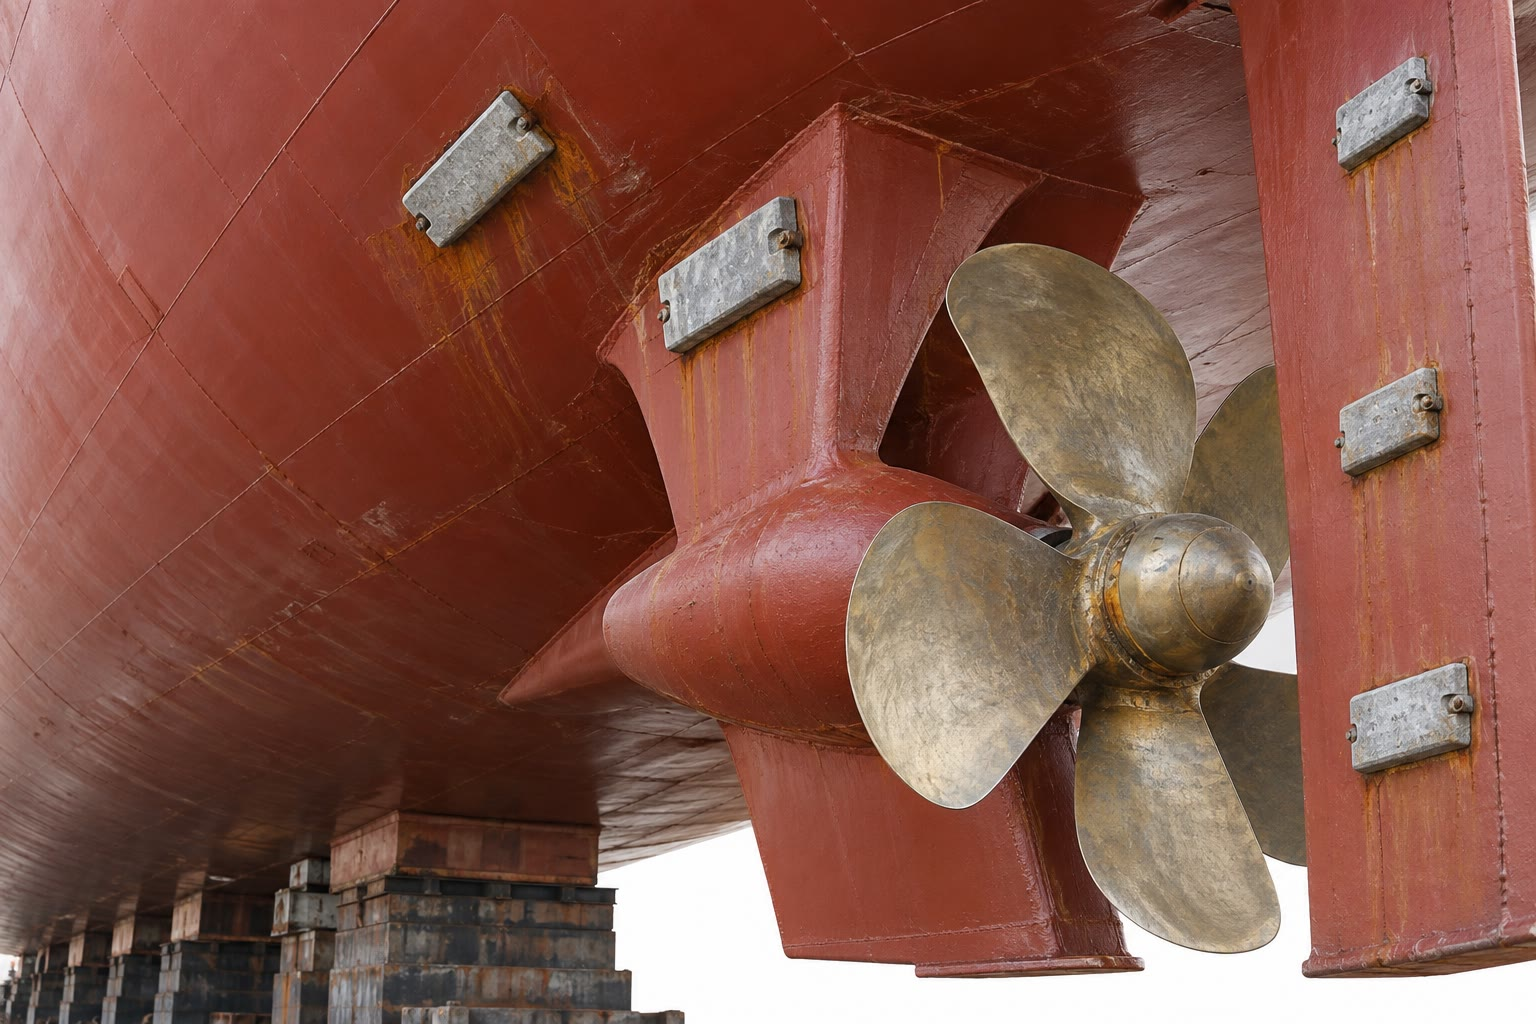
\includegraphics[width=0.6\linewidth]{images/book2/ai/b1-14-ship-anodes.jpg}

{\small La poupe d'un navire en cale sèche. Les blocs gris fixés sur la
coque près de l'hélice sont en zinc~: dans l'eau de mer, ils se corrodent
à la place de l'acier (\cref{exo:b1:e-ph-diagrams:12}).}
\end{omfigure}

\section{Conventions}

\begin{definition}[Diagramme potentiel--pH, concentration de tracé]\label{def:b1:e-ph-diagrams:e-ph-diagram}
Le \emph{diagramme potentiel--pH}\index{diagramme potentiel--pH} d'un
élément est le plan $(\mathrm{pH}, E)$ partagé en régions, chacune étant
le domaine de prédominance (espèces dissoutes) ou d'existence (solides)
d'une forme de l'élément. On le trace pour une \emph{concentration de
tracé}\index{concentration de trace@concentration de tracé} $c$ choisie, la concentration totale de
l'élément en solution, avec les conventions suivantes~:
\begin{itemize}
  \item sur une frontière entre deux espèces dissoutes, chacune est à la
        concentration $c$ (comptée en atomes de l'élément)~;
  \item sur une frontière entre une espèce dissoute et un solide,
        l'espèce dissoute est à la concentration $c$ et le solide est
        tout juste présent~;
  \item les gaz sont sous \qty{1}{bar}.
\end{itemize}
Dans ce chapitre, $c = \qty{0.010}{mol/L}$.
\end{definition}

Les formes de l'élément sont rangées par \omterm{def:b1:nernst:oxidation-number}{nombre d'oxydation}~: plus il
est élevé, plus la forme est haut sur le diagramme (les formes oxydées
sont stables à potentiel élevé). À \omterm{def:b1:nernst:oxidation-number}{nombre d'oxydation} donné, les formes
les plus basiques (hydroxydes, oxydes, \omterm{def:b1:complexation:complex}{complexes} hydroxo) sont à droite.

\begin{proposition}[Pente d'une frontière]\label{prop:b1:e-ph-diagrams:boundary-slope}
Une frontière entre deux espèces de \omterm{def:b1:nernst:oxidation-number}{nombres d'oxydation} différents, dont
la \omterm{def:b1:nernst:couple}{demi-équation} échange $n$ électrons et $m$ protons,
$\mathrm{Ox} + m\,\ce{H+} + n\,\mathrm{e^-} \rightleftharpoons \mathrm{Red} +
\cdots$, est une droite de pente $-0.059\,m/n$ volt par unité de pH. Une
frontière entre deux espèces de même \omterm{def:b1:nernst:oxidation-number}{nombre d'oxydation} est verticale.
\end{proposition}

\begin{proof}
La \omterm{thm:b1:nernst:nernst}{relation de Nernst} donne $E = E^\circ + \frac{0.059}{n}\log\frac{[\mathrm{Ox}]
[\ce{H+}]^m}{[\mathrm{Red}]} = E^\circ + \frac{0.059}{n}\log\frac{[\mathrm{Ox}]}
{[\mathrm{Red}]} - \frac{0.059\,m}{n}\,\mathrm{pH}$, et sur la frontière
les concentrations sont fixées par les conventions. Deux espèces de même
\omterm{def:b1:nernst:oxidation-number}{nombre d'oxydation} sont reliées par un équilibre acido-basique ou de
précipitation sans électrons, dont la constante fixe le pH de la
frontière quel que soit le potentiel.
\end{proof}

\section{L'eau}

\begin{proposition}[Les deux droites de l'eau]\label{prop:b1:e-ph-diagrams:water-lines}
Sous \qty{1}{bar} de gaz, l'eau est réduite en dihydrogène au-dessous de
la droite
$E = -0.059\,\mathrm{pH}$ et oxydée en dioxygène au-dessus de la droite $E = 1.23
- 0.059\,\mathrm{pH}$.
\end{proposition}

\begin{proof}
\ce{2H+ + 2e- -> H2}~: $E = 0 + \frac{0.059}{2}\log\frac{[\ce{H+}]^2}{p(\ce{H2})}
= -0.059\,\mathrm{pH}$ pour $p = 1$. \ce{O2 + 4H+ + 4e- -> 2H2O}~: $E = 1.23 +
\frac{0.059}{4}\log(p(\ce{O2})[\ce{H+}]^4) = 1.23 - 0.059\,\mathrm{pH}$.
Au-dessous de la première droite, \ce{H2} est la forme stable du couple
(l'eau est réduite)~; au-dessus de la seconde, c'est \ce{O2}.
\end{proof}

\begin{definition}[Domaine de stabilité de l'eau]\label{def:b1:e-ph-diagrams:water-domain}
La bande comprise entre les deux droites, large de \qty{1.23}{V} à tout
pH, est le \emph{domaine de stabilité de l'eau}\index{domaine de stabilite de l'eau@domaine de stabilité de l'eau}~: une
espèce dont le domaine est entièrement inclus dans cette bande n'oxyde
ni ne réduit l'eau.
\end{definition}

\section{Construire un diagramme~: le fer}

\begin{method}[Construire un diagramme potentiel--pH]\label{met:b1:e-ph-diagrams:build}
\begin{enumerate}
  \item Recenser les espèces et les classer par \omterm{def:b1:nernst:oxidation-number}{nombre d'oxydation}~:
        pour le fer, \ce{Fe} (0), \ce{Fe^2+} et \ce{Fe(OH)2} ($+$II),
        \ce{Fe^3+} et \ce{Fe(OH)3} ($+$III).
  \item À chaque \omterm{def:b1:nernst:oxidation-number}{nombre d'oxydation}, trouver les frontières verticales à
        partir des équilibres de précipitation (ou acido-basiques) à la
        \omterm{def:b1:e-ph-diagrams:e-ph-diagram}{concentration de tracé} (\cref{ch:b1:precipitation}).
  \item Pour chaque paire de \omterm{def:b1:nernst:oxidation-number}{nombres d'oxydation} voisins, écrire la
        \omterm{def:b1:nernst:couple}{demi-équation} dans chaque domaine de pH et sa \omterm{thm:b1:nernst:nernst}{relation de Nernst}
        avec les conventions~; on obtient une frontière rectiligne de
        pente connue.
  \item Assembler les droites de gauche à droite~; là où trois droites
        se rencontrent, chacune ne se poursuit que du côté où ses deux
        espèces sont stables.
  \item Vérifier~: les domaines ne doivent pas se chevaucher, et les
        pentes doivent être conformes à la
        \cref{prop:b1:e-ph-diagrams:boundary-slope}.
\end{enumerate}
\end{method}

\begin{example}[Les frontières du fer]\label{ex:b1:e-ph-diagrams:iron}
Avec $c = \qty{0.010}{mol/L}$ (et les constantes des \cref{ch:b1:precipitation,ch:b1:nernst})~:
\begin{itemize}
  \item \ce{Fe^3+}/\ce{Fe(OH)3}~: $\mathrm{pH} = 14.00 - \frac13(38.55 - 2) = 1.82$;
        \ce{Fe^2+}/\ce{Fe(OH)2}~: $\mathrm{pH} = 14.00 - \frac12(16.31 - 2) = 6.85$.
  \item \ce{Fe^2+}/\ce{Fe}~: $E = -0.41 + 0.030\log c = -0.47$~V (pH
        inférieur à 6.85).
  \item \ce{Fe^3+}/\ce{Fe^2+}~: $E = 0.77$~V (tous deux à $c$, pH
        inférieur à 1.82).
  \item \ce{Fe(OH)3}/\ce{Fe^2+}~: \ce{Fe(OH)3 + 3H+ + e- -> Fe^2+ + 3H2O},
        pente
        $-0.177$~: $E = 1.09 - 0.177\,\mathrm{pH}$ entre pH 1.82 et 6.85.
  \item \ce{Fe(OH)3}/\ce{Fe(OH)2}~: un électron, un proton, $E = 0.28 -
        0.059\,\mathrm{pH}$~; \ce{Fe(OH)2}/\ce{Fe}~: deux électrons, deux
        protons, $E = -0.07 - 0.059\,\mathrm{pH}$ (pH supérieur à 6.85).
\end{itemize}
Les ordonnées à l'origine s'obtiennent par continuité aux points
triples, ou directement à partir des enthalpies libres de formation~; le
diagramme ci-dessous est calculé à partir de ces dernières, et ses
frontières diffèrent de ces valeurs arrondies de moins de \qty{0.01}{V}
ou de 0.01 unité de pH.
% ledger: dfg:Fe2+_ao, dfg:Fe3+_ao, dfg:Fe_OH2_cr, dfg:Fe_OH3_cr, dfg:H2O_l, dfg:OH-_ao (boundaries computed in figdata/bachelor-1/eph-diagrams.py)
\end{example}

\begin{omfigure}
\begin{tikzpicture}
\begin{axis}[
  width=0.8\linewidth, height=8.2cm, xmin=0, xmax=14, ymin=-1.2, ymax=1.6,
  axis x line=bottom, axis y line=left, xlabel={pH}, ylabel={$E$ (V)},
  xtick={0,2,4,6,8,10,12,14}, ytick={-1,-0.5,0,0.5,1,1.5},
  unbounded coords=jump, clip=true,
  tick label style={font=\small}, label style={font=\small}]
\addplot[black!45, dashed] table[x=pH, y=H2] {figdata/out/bachelor-1-eph-diagrams-water.dat};
\addplot[black!45, dashed] table[x=pH, y=O2] {figdata/out/bachelor-1-eph-diagrams-water.dat};
\addplot[omDef, very thick] table[x=pH, y=E] {figdata/out/bachelor-1-eph-diagrams-iron.dat};
\node[font=\small] at (axis cs:3.2,-0.85) {\ce{Fe}};
\node[font=\small] at (axis cs:3.4,0.15) {\ce{Fe^2+}};
\node[font=\small] at (axis cs:0.9,1.45) {\ce{Fe^3+}};
\node[font=\small] at (axis cs:8.5,0.25) {\ce{Fe(OH)3}};
\node[font=\scriptsize] at (axis cs:11.0,-0.56) {\ce{Fe(OH)2}};
\node[font=\scriptsize, black!55, rotate=-14, anchor=south] at (axis cs:12.0,0.52) {\ce{O2}/\ce{H2O}};
\node[font=\scriptsize, black!55, rotate=-14, anchor=south] at (axis cs:2.2,-0.11) {\ce{H2O}/\ce{H2}};
\end{axis}
\end{tikzpicture}

{\small \omterm{def:b1:e-ph-diagrams:e-ph-diagram}{Diagramme potentiel--pH} du fer pour $c = \qty{0.010}{mol/L}$
(traits pleins), avec les deux droites de l'eau (tirets). Chaque
frontière est calculée à partir des enthalpies libres de formation
tabulées.}
\end{omfigure}

\section{Le cuivre et le zinc}

La même méthode donne les diagrammes du cuivre (espèces \ce{Cu},
\ce{Cu+}, \ce{Cu2O} à $+$I, \ce{Cu^2+}, \ce{CuO} à $+$II) et du zinc
(\ce{Zn}, \ce{Zn^2+}, \ce{Zn(OH)2}, \ce{Zn(OH)4^2-}). Pour le cuivre,
\ce{CuO} apparaît à $\mathrm{pH} = 14.00 - \frac12(20.64 - 2) = 4.68$,
et l'ion \ce{Cu+}, bien que recensé, n'a aucun domaine~: en milieu acide,
$E^\circ(\ce{Cu+}/\ce{Cu}) = 0.52$~V est au-dessus de
$E^\circ(\ce{Cu^2+}/\ce{Cu+}) = 0.16$~V, si bien que son domaine
potentiel est effacé par ses deux voisins
(\cref{sec:b1:e-ph-diagrams:reading}). Pour le zinc, l'hydroxyde apparaît
à pH 6.81 et ne se redissout en \ce{Zn(OH)4^2-} qu'au-dessus de 13.97 à
cette concentration~: une mince bande au bord droit.

\begin{omfigure}
\begin{tikzpicture}
\begin{axis}[name=cu,
  width=0.47\linewidth, height=7cm, xmin=0, xmax=14, ymin=-1.4, ymax=1.6,
  axis x line=bottom, axis y line=left, xlabel={pH}, ylabel={$E$ (V)},
  xtick={0,4,8,12}, ytick={-1,-0.5,0,0.5,1,1.5},
  unbounded coords=jump, clip=true,
  tick label style={font=\small}, label style={font=\small}]
\addplot[black!45, dashed] table[x=pH, y=H2] {figdata/out/bachelor-1-eph-diagrams-water.dat};
\addplot[black!45, dashed] table[x=pH, y=O2] {figdata/out/bachelor-1-eph-diagrams-water.dat};
\addplot[omDef, very thick] table[x=pH, y=E] {figdata/out/bachelor-1-eph-diagrams-copper.dat};
\node[font=\small] at (axis cs:5,-0.7) {\ce{Cu}};
\node[font=\small] at (axis cs:2,0.7) {\ce{Cu^2+}};
\node[font=\small] at (axis cs:9.5,0.75) {\ce{CuO}};
\node[font=\scriptsize] (cuo) at (axis cs:11.8,-1.05) {\ce{Cu2O}};
\draw[->, black!70] (cuo.north) -- (axis cs:10,-0.035);
\node[font=\small, anchor=north] at (axis cs:7,1.58) {cuivre};
\end{axis}
\begin{axis}[at={(cu.east)}, anchor=west, xshift=1.5cm,
  width=0.47\linewidth, height=7cm, xmin=0, xmax=14, ymin=-1.4, ymax=1.6,
  axis x line=bottom, axis y line=left, xlabel={pH}, ylabel={$E$ (V)},
  xtick={0,4,8,12}, ytick={-1,-0.5,0,0.5,1,1.5},
  unbounded coords=jump, clip=true,
  tick label style={font=\small}, label style={font=\small}]
\addplot[black!45, dashed] table[x=pH, y=H2] {figdata/out/bachelor-1-eph-diagrams-water.dat};
\addplot[black!45, dashed] table[x=pH, y=O2] {figdata/out/bachelor-1-eph-diagrams-water.dat};
\addplot[omDef, very thick] table[x=pH, y=E] {figdata/out/bachelor-1-eph-diagrams-zinc.dat};
\node[font=\small] at (axis cs:3.5,-1.15) {\ce{Zn}};
\node[font=\small] at (axis cs:3.2,0.4) {\ce{Zn^2+}};
\node[font=\small] at (axis cs:10.2,0.4) {\ce{Zn(OH)2}};
\draw[->] (axis cs:12.4,1.15) node[left, font=\scriptsize] {\ce{Zn(OH)4^2-}} -- (axis cs:13.95,1.15);
\node[font=\small, anchor=north] at (axis cs:10.5,1.58) {zinc};
\end{axis}
\end{tikzpicture}

{\small \omterm{def:b1:e-ph-diagrams:e-ph-diagram}{Diagrammes potentiel--pH} du cuivre et du zinc ($c =
\qty{0.010}{mol/L}$), avec les droites de l'eau (tirets). Le domaine du
cuivre métallique chevauche celui de l'eau~; celui du zinc est
entièrement situé au-dessous de la droite du dihydrogène.}
% ledger: dfg:Cu+_ao, dfg:Cu2+_ao, dfg:Cu2O_cr, dfg:CuO_cr, dfg:Zn2+_ao, dfg:Zn_OH2_cr, dfg:Zn_OH42-_ao (boundaries computed in figdata/bachelor-1/eph-diagrams.py)
\end{omfigure}

\section{Lire un diagramme}\label{sec:b1:e-ph-diagrams:reading}

\begin{proposition}[Domaines disjoints]\label{prop:b1:e-ph-diagrams:disjoint-domains}
Si, à un pH donné, le domaine d'un \omterm{def:b1:nernst:couple}{oxydant} est entièrement au-dessus de
celui d'un \omterm{def:b1:nernst:couple}{réducteur}, sans partie commune, les deux réagissent~; des
espèces dont les domaines ont une région commune peuvent coexister à
l'équilibre.
\end{proposition}

\begin{proof}
À ce pH, au-dessus de sa frontière, le couple de l'\omterm{def:b1:nernst:couple}{oxydant} a un potentiel
supérieur à tous ceux que peut atteindre le couple du \omterm{def:b1:nernst:couple}{réducteur}~:
d'après la \cref{prop:b1:nernst:equilibrium-constant}, la réaction entre
eux a une constante
$K > 1$, et elle se poursuit jusqu'à ce que l'un d'eux soit épuisé ou que
leurs domaines se rejoignent. Dans une région commune, les deux espèces
sont les formes stables au même potentiel~: rien ne pousse à une
réaction.
\end{proof}

Le fer et l'eau~: le domaine du fer métallique est au-dessous de la
droite \ce{H2O}/\ce{H2} à tout pH. Le fer réduit l'eau, en solution
acide avec un dégagement visible de dihydrogène~; en présence de
dioxygène dissous, il est oxydé plus vite encore. Le cuivre~: son domaine
chevauche celui de l'eau, si bien que le cuivre ne réduit ni l'eau ni
les acides qui ne sont pas eux-mêmes \omterm{def:b1:nernst:couple}{oxydants}, mais le dioxygène de
l'air, au-dessus, l'oxyde lentement --- la patine verte des toits est un
produit ultérieur de cette oxydation, avec le dioxyde de carbone et des
composés soufrés. Un diagramme dit ce qui est possible, pas à quelle
vitesse~: bien des réactions qu'il permet sont lentes, question traitée
dans le volume de deuxième année.

\begin{definition}[Dismutation, médiamutation]\label{def:b1:e-ph-diagrams:disproportionation}
La \emph{dismutation}\index{dismutation} est la réaction d'une espèce
sur elle-même, une partie étant oxydée et l'autre réduite~:
\ce{2Cu+ -> Cu^2+ + Cu}. La réaction inverse, dans laquelle deux espèces
d'un même élément en donnent une de \omterm{def:b1:nernst:oxidation-number}{nombre d'oxydation} intermédiaire, est
la \emph{médiamutation}\index{mediamutation@médiamutation}~:
\ce{2Fe^3+ + Fe -> 3Fe^2+}.
\end{definition}

\begin{proposition}[Critère de dismutation]\label{prop:b1:e-ph-diagrams:disproportionation-criterion}
Une espèce B de \omterm{def:b1:nernst:oxidation-number}{nombre d'oxydation} intermédiaire, dans les couples A/B et
B/C, se dismute si $E(\mathrm{B}/\mathrm{C}) > E(\mathrm{A}/\mathrm{B})$~:
elle n'a alors pas de domaine propre, et une frontière unique A/C
remplace les deux.
\end{proposition}

\begin{proof}
B est l'\omterm{def:b1:nernst:couple}{oxydant} de B/C et le \omterm{def:b1:nernst:couple}{réducteur} de A/B. Si le couple B/C est
au-dessus de A/B, la règle du gamma (\cref{met:b1:nernst:predict-redox})
fait réagir B (\omterm{def:b1:nernst:couple}{oxydant}, couple supérieur) avec B (\omterm{def:b1:nernst:couple}{réducteur}, couple
inférieur), ce qui donne C et A. Géométriquement, B ne serait stable
qu'au-dessus de $E(\mathrm{B}/\mathrm{C})$
et au-dessous de $E(\mathrm{A}/\mathrm{B})$~: un ensemble vide.
\end{proof}

\begin{definition}[Domaines d'immunité, de corrosion et de passivation]\label{def:b1:e-ph-diagrams:corrosion-domains}
Sur le diagramme d'un métal, le domaine du métal lui-même est son
\emph{domaine d'immunité}\index{domaine d'immunite@domaine d'immunité} (il ne peut pas être oxydé)~;
les domaines de ses ions dissous forment le \emph{domaine de
corrosion}\index{domaine de corrosion}~; les domaines de ses oxydes et
hydroxydes solides, qui peuvent recouvrir le métal, forment le
\emph{domaine de passivation}\index{domaine de passivation}. Savoir si
une couche protège réellement le métal est une question de cinétique,
traitée dans le volume de deuxième année.
\end{definition}

\begin{method}[Lire un diagramme]\label{met:b1:e-ph-diagrams:read}
\begin{enumerate}
  \item Superposer les droites de l'eau~: une espèce dont le domaine est
        hors de la bande de l'eau réagit avec l'eau
        (thermodynamiquement).
  \item Pour deux espèces d'éléments différents, superposer leurs
        diagrammes~: des domaines disjoints au pH considéré signifient
        une réaction.
  \item Pour un métal, placer le point (pH, $E$) du milieu~: immunité,
        corrosion ou passivation.
  \item Se rappeler qu'un diagramme est tracé pour une seule
        \omterm{def:b1:e-ph-diagrams:e-ph-diagram}{concentration de tracé}~; les frontières faisant intervenir des
        espèces dissoutes se déplacent de $0.059/n$~V par décade de
        concentration.
\end{enumerate}
\end{method}

Le zinc protège le fer~: dans l'eau de mer (pH 8 environ), le zinc et
l'acier d'une coque sont en contact~; le zinc, de potentiel plus bas,
est oxydé le premier, et les électrons qu'il libère maintiennent le fer
dans son \omterm{def:b1:e-ph-diagrams:corrosion-domains}{domaine d'immunité} ou près de lui. Le bloc de zinc s'use et
est remplacé à chaque passage en cale sèche.

\section{Exercices}

\begin{exercise}[$\star$]\label{exo:b1:e-ph-diagrams:1}
Classer par \omterm{def:b1:nernst:oxidation-number}{nombre d'oxydation} de l'élément les espèces \ce{Mn},
\ce{Mn^2+}, \ce{MnO2}, \ce{MnO4-}, \ce{Mn(OH)2}, ainsi que \ce{Cl-},
\ce{Cl2}, \ce{HClO},
\ce{ClO-}, \ce{ClO3-}.
\end{exercise}

\begin{exercise}[$\star$]\label{exo:b1:e-ph-diagrams:2}
Donner la pente de la frontière pour chaque \omterm{def:b1:nernst:couple}{demi-équation}~:
\ce{Fe(OH)3 + 3H+ + e- -> Fe^2+ + 3H2O}~; \ce{2Cu^2+ + H2O + 2e- -> Cu2O + 2H+}~;
\ce{MnO4- + 8H+ + 5e- -> Mn^2+ + 4H2O}~; \ce{Zn(OH)2 + 2H+ + 2e- -> Zn + 2H2O}.
Pourquoi l'une d'elles a-t-elle une pente positive~?
\end{exercise}

\begin{exercise}[$\star$]\label{exo:b1:e-ph-diagrams:3}
À quel pH les droites de l'eau passent-elles par 0~V et par
\qty{0.50}{V}~? Quelle est la largeur du \omterm{def:b1:e-ph-diagrams:water-domain}{domaine de stabilité de l'eau} à
pH 7~?
\end{exercise}

\begin{exercise}[$\star$]\label{exo:b1:e-ph-diagrams:4}
À l'aide du diagramme du fer, donner la forme stable du fer en
(pH 1, $E = 1.0$~V), (pH 4, $E = 0$), (pH 10, $E = -0.4$~V) et
(pH 10, $E = 0.5$~V).
\end{exercise}

\begin{exercise}[$\star\star$]\label{exo:b1:e-ph-diagrams:5}
Recalculer la frontière \ce{Fe^2+}/\ce{Fe} et la verticale
\ce{Fe^3+}/\ce{Fe(OH)3} pour une \omterm{def:b1:e-ph-diagrams:e-ph-diagram}{concentration de tracé} de
\qty{1.0e-6}{mol/L}, valeur retenue pour discuter de la corrosion. Quels
domaines s'agrandissent~?
\end{exercise}

\begin{exercise}[$\star\star$]\label{exo:b1:e-ph-diagrams:6}
Établir la frontière \ce{Fe(OH)3}/\ce{Fe^2+}~: écrire la \omterm{def:b1:nernst:couple}{demi-équation},
sa \omterm{thm:b1:nernst:nernst}{relation de Nernst}, et utiliser la continuité à pH 1.82 pour montrer
que $E = 1.09 -
0.177\,\mathrm{pH}$.
\end{exercise}

\begin{exercise}[$\star\star$]\label{exo:b1:e-ph-diagrams:7}
Montrer à l'aide du tableau des \omterm{def:b1:nernst:electrode-potential}{potentiels standard} que \ce{Cu+} se
dismute à pH 0 et donner le potentiel de la frontière unique
\ce{Cu^2+}/\ce{Cu} pour $c = \qty{0.010}{mol/L}$.
\end{exercise}

\begin{exercise}[$\star\star$]\label{exo:b1:e-ph-diagrams:8}
Le cuivre se dissout-il dans l'acide chlorhydrique à pH 0 en l'absence
d'air~? dans l'acide nitrique (couple \ce{NO3-}/\ce{NO},
$E^\circ = 0.96$~V)~? Justifier à l'aide du diagramme et des potentiels.
\end{exercise}

\begin{exercise}[$\star\star$]\label{exo:b1:e-ph-diagrams:9}
Les solutions de fer(II) laissées à l'air jaunissent puis brunissent.
Expliquer à l'aide du diagramme du fer et de la droite
\ce{O2}/\ce{H2O}, et écrire la réaction à pH 3.
\end{exercise}

\begin{exercise}[$\star\star\star$]\label{exo:b1:e-ph-diagrams:10}
Construire le diagramme du zinc pour $c = \qty{0.010}{mol/L}$~: calculer
les frontières verticales à pH 6.81 et 13.97, la frontière
\ce{Zn^2+}/\ce{Zn}, et les équations de \ce{Zn(OH)2}/\ce{Zn} et de
\ce{Zn(OH)4^2-}/\ce{Zn}.
\end{exercise}

\begin{exercise}[$\star\star\star$]\label{exo:b1:e-ph-diagrams:11}
Superposer les diagrammes du fer et de l'eau et discuter du sort d'un
clou en fer dans une eau désoxygénée à pH 2, à pH 7 et à pH 13. Qu'est-ce
qui change en présence de dioxygène dissous~?
\end{exercise}

\begin{exercise}[$\star\star\star$]\label{exo:b1:e-ph-diagrams:12}
\omterm{def:b1:nernst:cell}{Anodes} sacrificielles. Une coque d'acier dans l'eau de mer (pH 8) est
reliée à un bloc de zinc. À l'aide des diagrammes, expliquer quel métal
est oxydé, écrire les réactions avec le dioxygène dissous, et dire
pourquoi le magnésium conviendrait aussi et le cuivre aggraverait les
choses.
\end{exercise}

\section{Problème~: l'eau de Javel et la piscine}

\begin{problem}[{Problème du week-end --- \omterm{def:b1:nernst:oxidation-number}{nombres d'oxydation} du chlore,
le \omterm{def:b1:predominant-reaction:bronsted}{couple acide/base} HClO/ClO\textsuperscript{$-$}, le \omterm{def:b1:e-ph-diagrams:e-ph-diagram}{diagramme
potentiel--pH} du chlore, et le pH au-dessus duquel le dichlore dissous
se dismute}]
\label{pb:b1:e-ph-diagrams:1}
L'eau de Javel est une solution basique d'hypochlorite de sodium et de
chlorure de sodium~; une piscine est désinfectée par l'acide
hypochloreux qu'elle contient, à un pH maintenu un peu au-dessus de 7.
Mélanger de l'eau de Javel avec un détartrant acide libère du dichlore
gazeux. Données à \qty{25}{\celsius}~: $E^\circ(\ce{Cl2(aq)}/\ce{Cl-})
= 1.396$~V, $E^\circ(\ce{HClO}/\ce{Cl2(aq)}) = 1.594$~V,
$\mathrm{p}K_a(\ce{HClO}/\ce{ClO-}) = 7.55$, $RT\ln 10/F = 0.0592$~V~;
\omterm{def:b1:e-ph-diagrams:e-ph-diagram}{concentration de tracé} $c = \qty{0.010}{mol/L}$ en atomes de chlore.

\medskip
\noindent\textbf{Partie I --- Les espèces.}
\begin{enumerate}
  \item Donner le \omterm{def:b1:nernst:oxidation-number}{nombre d'oxydation} du chlore dans \ce{Cl-}, \ce{Cl2},
        \ce{HClO} et \ce{ClO-}.
  \item Classer les quatre espèces sur un axe vertical des \omterm{def:b1:nernst:oxidation-number}{nombres
        d'oxydation}.
  \item Quelles espèces ont le même \omterm{def:b1:nernst:oxidation-number}{nombre d'oxydation}~? Comment
        sont-elles reliées~?
  \item Écrire la \omterm{def:b1:nernst:couple}{demi-équation} de \ce{Cl2}/\ce{Cl-}.
  \item Écrire la \omterm{def:b1:nernst:couple}{demi-équation} de \ce{HClO}/\ce{Cl2}.
  \item Écrire la \omterm{def:b1:nernst:couple}{demi-équation} de \ce{ClO-}/\ce{Cl-} en solution basique.
\end{enumerate}

\medskip
\noindent\textbf{Partie II --- L'acide hypochloreux.}
\begin{enumerate}[resume]
  \item Tracer le \omterm{def:b1:predominant-reaction:predominance}{diagramme de prédominance} de \ce{HClO} et de \ce{ClO-}
        en fonction du pH.
  \item Pourquoi leur frontière sur le \omterm{def:b1:e-ph-diagrams:e-ph-diagram}{diagramme potentiel--pH} est-elle
        verticale~?
  \item Calculer la fraction d'acide hypochloreux à pH 7.4.
  \item Même question à pH 8.0. L'acide hypochloreux est le meilleur
        désinfectant~: pourquoi les exploitants de piscines empêchent-ils
        le pH de dériver jusqu'à 8~?
  \item Dans l'eau de Javel (pH 12 environ), quelle forme est présente~?
\end{enumerate}

\medskip
\noindent\textbf{Partie III --- Le diagramme.}
Avec les conventions du chapitre, \ce{Cl2(aq)} est à $c/2$ et \ce{Cl-},
\ce{HClO}, \ce{ClO-} à $c$ sur une frontière.
\begin{enumerate}[resume]
  \item Montrer que la frontière \ce{Cl2}/\ce{Cl-} se situe à $E = 1.396 +
        0.0296\log\bigl((c/2)/c^2\bigr) = 1.446$~V, indépendamment du pH.
  \item Montrer que la frontière \ce{HClO}/\ce{Cl2} a pour équation
        $E = 1.594 -
        0.0296\log 50 - 0.0592\,\mathrm{pH} \approx 1.544 -
        0.0592\,\mathrm{pH}$.
  \item Trouver le pH où ces deux droites se coupent.
  \item Au-delà de ce pH, la frontière est \ce{HClO}/\ce{Cl-}. Écrire sa
        \omterm{def:b1:nernst:couple}{demi-équation} et montrer que sa pente vaut $-0.0296$.
  \item Calculer $E^\circ(\ce{HClO}/\ce{Cl-})$ à partir des deux
        potentiels donnés.
  \item Écrire la frontière \ce{ClO-}/\ce{Cl-} au-dessus de pH 7.55~;
        vérifier sa continuité à pH 7.55.
  \item Esquisser le diagramme de pH 0 à 14, avec la droite
        \ce{O2}/\ce{H2O}.
  \item L'acide hypochloreux est-il stable dans l'eau,
        thermodynamiquement~? Pourquoi une piscine n'a-t-elle pourtant
        besoin que de petits ajouts de chlore chaque jour~?
\end{enumerate}

\medskip
\noindent\textbf{Partie IV --- La \omterm{def:b1:e-ph-diagrams:disproportionation}{dismutation} et le danger des acides.}
\begin{enumerate}[resume]
  \item Au-dessus du pH de la question 14, que devient le dichlore
        dissous~? Écrire la réaction dans l'eau et en solution basique.
  \item Comment fabrique-t-on l'eau de Javel à partir du dichlore~?
  \item Au-dessous de ce même pH, écrire la réaction entre \ce{HClO} et
        \ce{Cl-}. Comment s'appelle-t-elle~?
  \item Un détartrant acide pour toilettes amène l'eau de Javel à pH 1.
        Que se passe-t-il~?
  \item Pourquoi le danger est-il moindre avec un produit faiblement
        acide (pH 4)~? Répondre à l'aide du diagramme, puis nuancer.
  \item Donner, à une décimale près, le pH au-dessus duquel le dichlore
        dissous se dismute pour $c = \qty{0.010}{mol/L}$.
\end{enumerate}
\end{problem}
